\documentclass[11pt,a4paper,twoside]{article}

% Input encoding and basic packages
\usepackage[utf8]{inputenc}
\usepackage{amsmath, amssymb}
\usepackage{graphicx}
\usepackage{tcolorbox}
\usepackage{xcolor}
\usepackage{geometry}
\usepackage{wrapfig}
\usepackage{titlesec}
\usepackage{fancyhdr}
\usepackage{caption}
\usepackage{float}
\usepackage{hyperref}
\usepackage{subcaption}
\usepackage{fontspec}
\usepackage{nomencl} 
\usepackage{multicol}
\usepackage{etoolbox}
\usepackage{sectsty} % Allows custom section styles
\usepackage{helvet}  % Default sans-serif font
\usepackage{times}   % Example serif font for body text

% Define custom fonts
\setmainfont{Poppins} % Main font for body text
\newfontfamily\titlesfont{Anonymous Pro} % Font for titles

% Relax Latex rules for text layout
\raggedbottom
\sloppy
\hbadness=10000


% Define custom colors
\definecolor{cherenkovblue}{RGB}{55, 139, 230}

% Adjust default font sizes (Explicitly set sizes)
\renewcommand{\normalsize}{\fontsize{9}{11}\selectfont} % Smaller body text: 9pt font with 11pt line spacing
\renewcommand{\small}{\fontsize{8}{10}\selectfont}
\renewcommand{\footnotesize}{\fontsize{7}{9}\selectfont}

% Make titles all caps
\makeatletter
\let\oldsection\section
\renewcommand{\section}{\@startsection {section}{1}{\z@}%
  {-3.5ex \@plus -1ex \@minus -.2ex}%
  {2.3ex \@plus.2ex}%
  {\titlesfont\fontsize{14}{16}\bfseries\color{cherenkovblue}\MakeUppercase}}
\makeatother

% Custom subsection font
\subsectionfont{\titlesfont\fontsize{12}{14}\bfseries\color{cherenkovblue}} % Subsection: 12pt font, bold, blue

% Customize spacing
\setlength{\parskip}{6pt} % Add spacing between paragraphs
\setlength{\parindent}{0pt} % Remove paragraph indentation
\setlength{\itemsep}{4pt} % Add spacing between list items

% Customize itemize bullets
\renewcommand\labelitemi{--} % Use dashes instead of bullets

% Define fancy header and footer
\fancypagestyle{plain}{
    \fancyhf{} % Clear all header and footer fields
} % Default plain style for title and index pages

\fancypagestyle{post-index}{
    \fancyhf{} % Clear all header and footer fields
    \fancyhead[LE]{\textit{S.Pagliuca, T.Pirola, L.Raffuzzi, R.Ronchi, D.Shabi}}
    \fancyhead[RO]{\textit{Nuclear Design and Technologies}}
    \fancyfoot[LE,RO]{\thepage}
    \renewcommand{\headrulewidth}{0.4pt}
    \renewcommand{\footrulewidth}{0.4pt}
    \setlength{\headheight}{14pt}
}

\begin{document}
%%%%%%%%%%%%%%%%%%%%%%%%%%%%%%%%%%%%%%%%%%%%%%%%%%%%%%%%%%%%%%%%%%%%%%%%%%%%%%%%%%%%%%%%%%%%
% First page
% Includes title, author, abstract, keywords, nomenclature
\thispagestyle{plain}

% Title with Titles Font (Anonymous Pro)
{\titlesfont\fontsize{18}{28}\textbf{\color{cherenkovblue}{FUEL PIN \\ PRELIMINARY DESIGN}}}\\
{\titlesfont\fontsize{10}{12}\color{cherenkovblue} Nuclear Engineering - Politecnico di Milano}\\


\vspace{-10pt}

% Author information with Main Font (Poppins)
{\normalsize\textbf{Simone Pagliuca, Tommaso Pirola, Lisa Raffuzzi, Riccardo Ronchi, Darien Shabi}} \\
{\footnotesize\textit{simone1.pagliuca@mail.polimi.it}} \\

\vspace{10pt}

% Course and Academic Year
{\footnotesize\textbf{Course:} Nuclear Design and Technologies}\\
{\footnotesize\textbf{Academic year:} 2024/2025}

% Horizontal rule
\vspace{8pt}
\centerline{\rule{1.0\textwidth}{0.4pt}}

\vspace{10pt}

% Abstract with Titles Font for Heading, Main Font for Body
{\fontsize{8}{8}\textbf{\color{cherenkovblue} ABSTRACT:}} 
{\normalsize
    lorem ipsum dolor sit amet, consectetur adipiscing elit. Donec auctor, nunc nec ultricies ultricies, nunc nunc.
}

\vspace{10pt}

% Key-words box with Titles Font
\begin{tcolorbox}[arc=0pt, boxrule=0pt, colback=cherenkovblue!60, width=\textwidth, colupper=white]
    {\titlesfont\fontsize{10}{10}\textbf{Key-words:}} Key, Words, Here
\end{tcolorbox}

\vspace{10pt}

% Nomenclature Definitions
\makenomenclature
\renewcommand\nomgroup[1]{%
\item[\bfseries
\ifstrequal{#1}{A}{A Quantities}{%
\ifstrequal{#1}{B}{B Quantities}{}}%
]}

% Two-column layout for the nomenclature
\renewcommand{\nompreamble}{\begin{multicols}{2}}
\renewcommand{\nompostamble}{\end{multicols}}

% Define Nomenclature Entries
\nomenclature[A, 01]{$x$}{X quantity}
\nomenclature[B]{$y$}{Y quantity}

% Render Nomenclature Without Section Break
\vspace{-5pt} % Adjust spacing to fit table
\printnomenclature

\newpage
%%%%%%%%%%%%%%%%%%%%%%%%%%%%%%%%%%%%%%%%%%%%%%%%%%%%%%%%%%%%%%%%%%%%%%%%%%%%%%%%%%%%%%%%%%%%

%%%%%%%%%%%%%%%%%%%%%%%%%%%%%%%%%%%%%%%%%%%%%%%%%%%%%%%%%%%%%%%%%%%%%%%%%%%%%%%%%%%%%%%%%%%%
% Table of contents
% it then switches to the post-index page style
\tableofcontents
\newpage
\pagestyle{post-index}
%%%%%%%%%%%%%%%%%%%%%%%%%%%%%%%%%%%%%%%%%%%%%%%%%%%%%%%%%%%%%%%%%%%%%%%%%%%%%%%%%%%%%%%%%%%%

%%%%%%%%%%%%%%%%%%%%%%%%%%%%%%%%%%%%%%%%%%%%%%%%%%%%%%%%%%%%%%%%%%%%%%%%%%%%%%%%%%%%%%%%%%%%
% Content
% Add files for content here

% INTRODUCTION

\section{Introduction}
This report presents the preliminary design and verification of a fuel pin for a sodium-cooled fast reactor, as specified in the assignment.

The analysis involves calculations for material properties, thermal-hydraulic conditions, and mechanical stress limits.

We verify the robustness of our models and justify the assumptions made throughout the process.
 % Chat

\section{Problem Description}
The fuel pin design problem requires:

\begin{itemize}
\item Determining the cladding thickness, fuel-cladding gap size, and plenum height.
\item Verifying the design against limits for fuel melting, cladding temperature, yielding, and rupture time.
\item Identifying critical aspects if irradiation time is doubled.
\end{itemize}

The project specifications and material properties are summarized in Table~\ref{tab:specs}.

\begin{table}[H]
\centering
\caption{Fuel pin design specifications.}
\label{tab:specs}

\includegraphics[width=0.8\textwidth]{placeholder.png}
\end{table}
 % Chat
\subsection{Assumptions}
To address the given problem, the following assumptions were made:

\textbf{Steady State Solution for Gas in Grains:}

\begin{itemize}
\item[$\hookrightarrow$] The rate equation for the gas remaining in the grains (PDE) was solved in steady state conditions, given that we just want to size the plenum for 1-year operation and are not interested in the specific behavior in time of the function.
\end{itemize}

\textbf{Fission Rate Calculation:}

\begin{itemize}
\item[$\hookrightarrow$] The fission rate was calculated by using the formula (macroscopic cross section * average flux).
\item[$\hookrightarrow$] The macroscopic cross section of fission was computed from data taken from the JANIS database.
\item[$\hookrightarrow$] The average flux was evaluated considering power and flux profile to be equal.
\end{itemize}

\textbf{Material Properties and Geometry:}

\begin{itemize}
\item[$\hookrightarrow$] Material properties are temperature-dependent and were modeled using provided empirical correlations.
\item[$\hookrightarrow$] Axial power and neutron flux profiles remain constant over time.
\item[$\hookrightarrow$] Initial helium pressure and temperature in the fuel-cladding gap were assumed as specified.
\item[$\hookrightarrow$] Simplifications in geometry, such as neglecting axial deformation, were made to ease computation.
\end{itemize}
 %

% VERIFICATION
\section{Verification of Models}
Each function used in the analysis was tested for expected behavior.

Below are the key verification steps.
\subsection{Thermal-Hydraulics Analysis}
Preliminary checks were conducted on coolant properties.

Density, viscosity, and thermal conductivity were validated at the coolant inlet temperature.

The heat transfer coefficient between the coolant and cladding was computed using Nusselt number correlations.

Figure~\ref{fig:thermal_hydraulics} shows the axial power profile. the computed heat transfer coefficient in cold geometry was $\alpha_{coolant} = 139.98 \frac{kW}{m^2 K}$.

\begin{figure}[H]
    \centering
    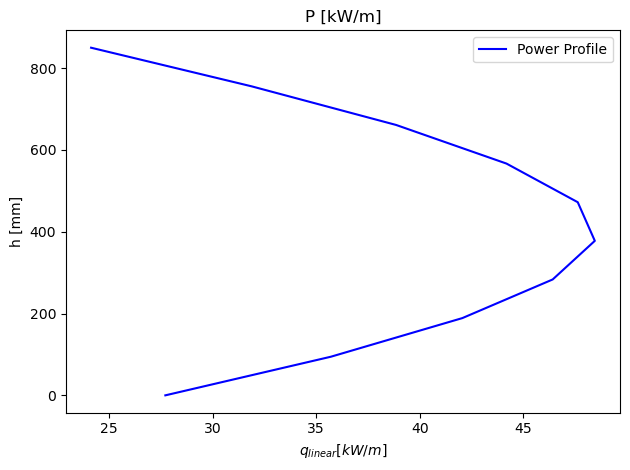
\includegraphics[width=0.8\textwidth]{power_profile.png}
    \caption{Thermal-hydraulics analysis results.}
    \label{fig:thermal_hydraulics}
    \end{figure} % Chat
\section{Temperature Profiles}
Radial and axial temperature profiles were computed for the cold geometry to verify the profile's shape and to ensure that the calculated values were reasonable.

A temperature map of the fuel rod was created. For each node along the axial direction, the temperature increase in the coolant was first computed based on the heat generated in the fuel. Using this, the temperature at the coolant-cladding interface was determined by applying the heat transfer coefficient, calculated from provided correlations.

For the cladding, a linear temperature profile was assumed to estimate the temperature at the cladding-gas interface. For the gap and the fuel, multiple temperature points were calculated along the radial direction. At each step, the material properties were updated to reflect the temperature of the previous step. The inner void was assumed to be at the same temperature as the inner surface of the fuel.

The results provided an initial validation of the temperature distribution behavior, confirming that the trends were consistent and the values were within expected ranges before proceeding with further analysis.

Figure~\ref{fig:axial_temp_profile} illustrates the axial temperature profile at the interfaces, while Figure~\ref{fig:radial_temp_profile} shows the radial temperature profiles at the bottom, middle, and top of the fuel rod.

\begin{figure}[H]
\centering
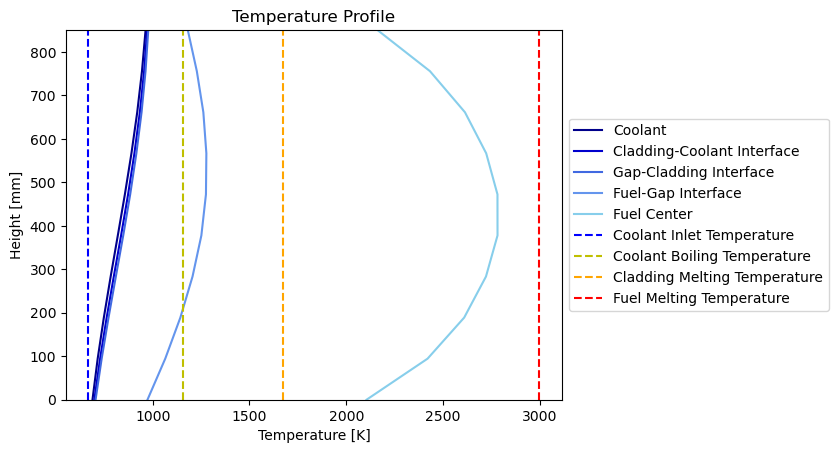
\includegraphics[width=0.7\textwidth]{axial_temp_profile_cold.png}
\caption{Axial temperature profile for cold geometry.}
\label{fig:axial_temp_profile}
\end{figure}

\begin{figure}[H]
\centering
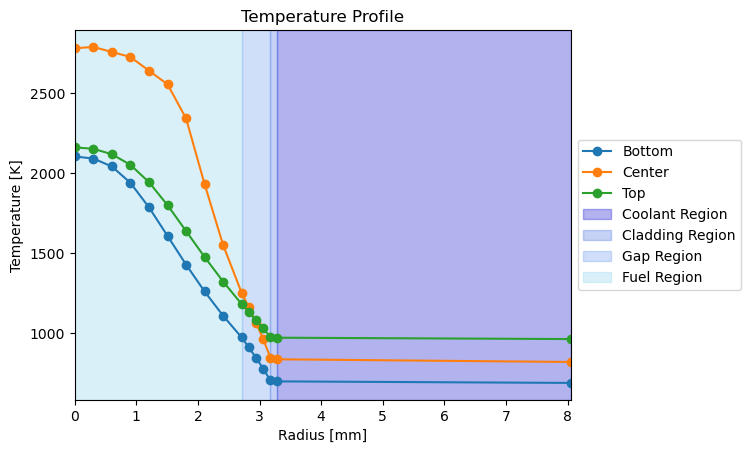
\includegraphics[width=0.7\textwidth]{radial_temp_profile_cold.png}
\caption{Radial temperature profiles for cold geometry at the bottom, middle, and top of the fuel rod.}
\label{fig:radial_temp_profile}
\end{figure}
 % Simo
\subsection{Thermal Expansion}
Figure \ref{fig:th_expansion} shows 

\begin{figure}[H]
\centering

\includegraphics[width=0.8\textwidth]{placeholder.png}
\caption{Cladding swelling due to void formation.}
\label{fig:th_expansion}
\end{figure}
 %
\subsection{Void Swelling}
The volumetric void swelling of the cladding was evaluated using a provided correlation. Assuming isotropic swelling, the radial expansion was estimated as one-third of the volumetric expansion:
\[
\Delta R_{\text{radial}} = \frac{1}{3} \Delta V_{\text{volumetric}}
\]

Figure~\ref{fig:void_swelling} illustrates the swelling of the cladding along the axial direction. As expected, swelling occurs only within a specific temperature range. At lower temperatures, swelling is negligible, while at higher temperatures, increased atomic mobility leads to recombination, which limits the extent of swelling.

\begin{figure}[H]
\centering
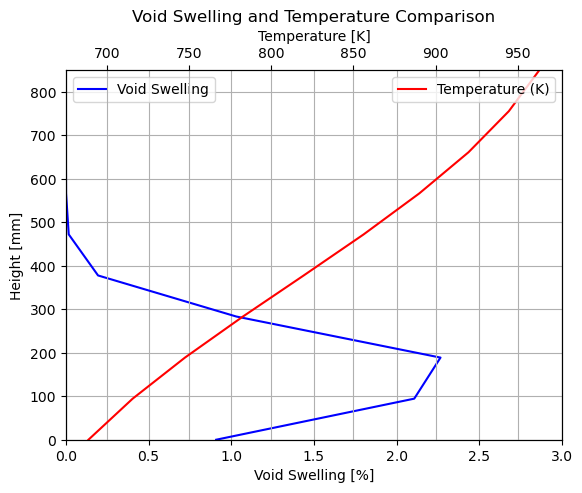
\includegraphics[width=0.8\textwidth]{void_swell.png}
\caption{Cladding swelling due to void formation along the axial direction.}
\label{fig:void_swelling}
\end{figure}
 % Simo
\subsection{Fission Gas Behavior}
Rate theory equations were solved to estimate fission gas production and release over the fuel cycle.

The rate equation for the gas remaining in the grains was solved under steady state conditions, given that we are only interested in sizing the plenum for 1-year operation.

The fission rate was calculated as the product of the macroscopic cross section and the average flux.

The macroscopic cross section was obtained from data in the JANIS database, and the average flux was estimated by assuming the power and flux profiles were equivalent.

The concentration profiles are shown in Figure~\ref{fig:fission_gas}.

\begin{figure}[H]
\centering

\includegraphics[width=0.8\textwidth]{placeholder.png}
\caption{Fission gas concentration profiles.}
\label{fig:fission_gas}
\end{figure} %
\section{Restructuring}
After transitioning from cold geometry to hot geometry and accounting for thermal expansion, the fuel restructuring process must be considered. This involves assumptions about the radii of columnar and equiaxed regions as well as the corresponding densities in these regions. According to Holander’s book, the temperature boundaries are set at 1800°C for the columnar region and 1600°C for the equiaxed region. Regarding densities, the as-fabricated region retains its original density, while the equiaxed region is assumed to have 95\% of the theoretical density (TD) and the columnar region 98\% of TD.

Initially, the columnar and equiaxed radii are evaluated at 1800°C and 1600°C, respectively, based on a temperature map. This map provides temperature values at various heights along the fuel pin and utilizes a precise function to determine the temperature at any position within the previously developed 3D model.

Once the columnar and equiaxed radii are determined, the void radius is calculated. The as-fabricated region corresponds to the remaining portion of the fuel outer radius after subtracting the equiaxed region. The following equation is used to estimate the void formation radius:
\begin{equation}
R_{\text{void}} = \sqrt{
    R_{\text{col}}^2 - R_{\text{eq}}^2 \cdot \left( \frac{\rho_{\text{AS}}}{\rho_{\text{col}}} \right)
    + \left( R_{\text{eq}}^2 - R_{\text{col}}^2 \right) \cdot \left( \frac{\rho_{\text{eq}}}{\rho_{\text{AS}}} \right)
}
\end{equation}

Finally, the relationship between height and radius is plotted to illustrate the restructuring phenomenon and highlight the axial position dependence (z-axis) of the fuel pin. Figure~\ref{fig:restructuring} shows the restructuring effect, with a particular focus on cladding swelling due to void formation.

\begin{figure}[H]
\centering
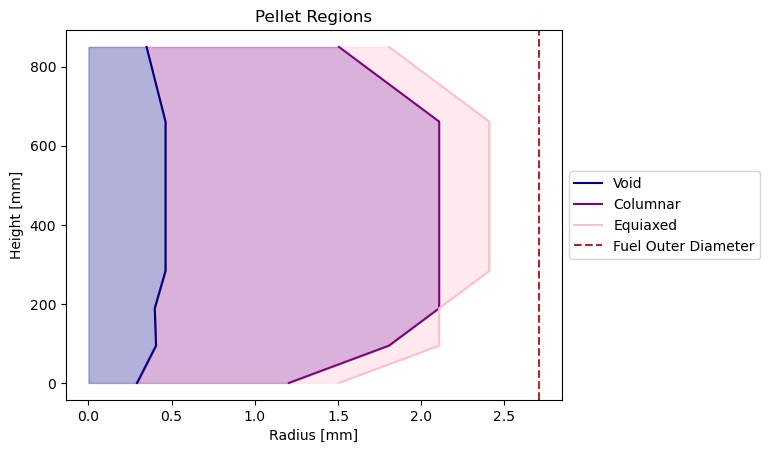
\includegraphics[width=0.8\textwidth]{restructuring.png}
\caption{Cladding swelling due to void formation.}
\label{fig:restructuring}
\end{figure}
 %
\section{Mechanical Analysis - Stress Assessment}

\subsection{Introduction}
This section focuses on the mechanical analysis of the cladding, evaluating stresses to ensure compliance with safety limits during operation. The analysis includes stress computations based on the Mariotte and Lamé criteria, an assessment of plastic strain potential, and an evaluation of rupture time due to thermal creep.

\subsection{Methodology}
The stress distribution in the cladding was calculated using elasticity equations for cylindrical geometries, under the assumptions of orthocylindricity and axial symmetry.

\subsubsection{Mariotte Criterion}
\begin{itemize}
    \item[$\hookrightarrow$] Evaluates the hoop stress at the mid-wall of the cladding.
    \item[$\hookrightarrow$] Used to check for yielding. Preliminary calculations indicated that the Mariotte stress is slightly higher than the Lamé stress, although the latter imposes stricter criteria.
\end{itemize}

\subsubsection{Lamé Criterion}
\begin{itemize}
    \item[$\hookrightarrow$] Considers radial, hoop, and axial stresses.
    \item[$\hookrightarrow$] The radial stress is computed using the pipe equation with a superposition solution:
    \begin{equation}
        \frac{d}{dr} \left( r^3 \cdot \frac{d\sigma_r(r)}{dr} \right) + \frac{\alpha E}{1 - \nu} \cdot \frac{dT(r)}{dr} = 0
    \end{equation}
    Using equilibrium relations, the hoop stress is determined as:
    \[
    \sigma_\theta = \sigma_r + \frac{d\sigma_r}{dr}
    \]
    \item[$\hookrightarrow$] The Tresca criterion is applied for verification, ensuring compliance with yield and ultimate strength limits. The Lamé criterion was found to impose limits approximately 33\% stricter than the Mariotte criterion.
\end{itemize}

\subsubsection{Plastic Strain Check}
\begin{itemize}
    \item[$\hookrightarrow$] Plastic strain is flagged if either criterion predicts stresses exceeding the yield strength.
    \item[$\hookrightarrow$] No significant plastic strain was observed when both criteria were satisfied.
\end{itemize}

\subsubsection{Thermal Creep (Time to Rupture)}
\begin{itemize}
    \item[$\hookrightarrow$] The rupture time due to thermal creep was evaluated using the Larson-Miller Parameter (LMP), based on operating stresses and temperatures.
    \item[$\hookrightarrow$] Even under conservative assumptions, the calculated time to rupture showed sufficient margins, indicating minimal risk of creep-related failure.
\end{itemize}

\subsection{Results and Conclusion}

\subsubsection{Stresses from Mariotte and Lamé}
\begin{itemize}
    \item[$\hookrightarrow$] Both criteria confirmed that the stresses remain below critical limits.
    \item[$\hookrightarrow$] While the Mariotte stress tends to be marginally higher, it remains within safe bounds. Lamé's stricter limits provide an additional safety margin.
\end{itemize}

\subsubsection{Plastic Strain}
\begin{itemize}
    \item[$\hookrightarrow$] No significant plastic strain was observed, confirming that the cladding operates within the elastic regime under specified conditions.
\end{itemize}

\subsubsection{Time to Rupture}
\begin{itemize}
    \item[$\hookrightarrow$] The LMP-based calculation indicated that the cladding's operational life significantly exceeds the irradiation period, even under conservative conditions.
\end{itemize}

These analyses validate the mechanical reliability of the cladding in the initial design. The results demonstrate that the proposed design is safe and robust, with sufficient margins for long-term operation. Further refinement of the design will allow for additional verification and optimization.
 %
\subsection{Helium Embrittlement}
Figure \ref{fig:he_embrittlment} shows the swelling of the cladding along the axial direction.

\begin{figure}[H]
\centering

\includegraphics[width=0.8\textwidth]{placeholder.png}
\caption{Cladding swelling due to void formation.}
\label{fig:he_embrittlment}
\end{figure}
 %

% DESIGN

\section{Plenum Design}
The relationship between plenum height and pressure was analyzed to ensure the pressure remains below 5~MPa.

Figure~\ref{fig:plenum_pressure} shows the results.

\begin{figure}[H]
\centering

\includegraphics[width=0.8\textwidth]{placeholder.png}
\caption{Plenum pressure as a function of height.}
\label{fig:plenum_pressure}
\end{figure}

 %

\section{Plenum Design}
The relationship between plenum height and pressure was analyzed to ensure the pressure remains below 5~MPa.

Figure~\ref{fig:plenum_pressure} shows the results.

\begin{figure}[H]
\centering

\includegraphics[width=0.8\textwidth]{placeholder.png}
\caption{Plenum pressure as a function of height.}
\label{fig:plenum_pressure}
\end{figure}

 %

% CONCLUSION

\section{Future Work}
In subsequent steps, we will develop a dimensioning loop to automate the iterative design process.

We will present final results, including optimized dimensions and safety margins, and comment on the design's robustness under extended irradiation.
 %
\appendix

\section{Code Listings}
Placeholder for code files.
 %
%%%%%%%%%%%%%%%%%%%%%%%%%%%%%%%%%%%%%%%%%%%%%%%%%%%%%%%%%%%%%%%%%%%%%%%%%%%%%%%%%%%%%%%%%%%%
\end{document}